\documentclass[urlcolor=blue,dvipsnames]{beamer}

\usepackage[utf8]{inputenc}
\usepackage{fancybox,fancyvrb}
\usepackage{environ,xspace}
\usepackage{tikz}
\hypersetup{colorlinks,linkcolor=,urlcolor=cyan}

\beamertemplatenavigationsymbolsempty
\setbeamertemplate{footline}[frame number]
\usetheme{Pittsburgh}

\newcommand\enumnum[1]{{\renewcommand{\insertenumlabel}{#1}%
      \usebeamertemplate{enumerate item} \,}}

\newcommand{\grad}{\nabla}
\newcommand{\ih}{\boldsymbol{\hat{\textbf{\i}}}}
\newcommand{\jh}{\boldsymbol{\hat{\textbf{\j}}}}
\newcommand{\vF}{\boldsymbol{\vec{\textbf{F}}}}
\newcommand{\Matlab}{\textsc{Matlab}\xspace}
\newcommand{\Octave}{\textsc{Octave}\xspace}


\title{6.2 Series solutions about ordinary points}

\subtitle{a lesson for MATH F302 Differential Equations}

\author{Ed Bueler, Dept.~of Mathematics and Statistics, UAF}

\date{\tiny \today}


\begin{document}
\setbeamertemplate{itemize item}{$\bullet$}
\setbeamertemplate{itemize subitem}{$\circ$}


\begin{frame}
\titlepage

\centerline{\tiny for textbook: \, D. Zill, \emph{A First Course in Differential Equations with Modeling Applications}, 11th ed.}
%\color{green!40!blue}
\end{frame}


\begin{frame}{Xs}

\begin{itemize}
\item X
\end{itemize}
\end{frame}


\begin{frame}{Airy equation}

\begin{itemize}
\item $y''+xy=0$
\end{itemize}
\end{frame}


\begin{frame}{Airy equation 2}

\begin{itemize}
\item X
\end{itemize}

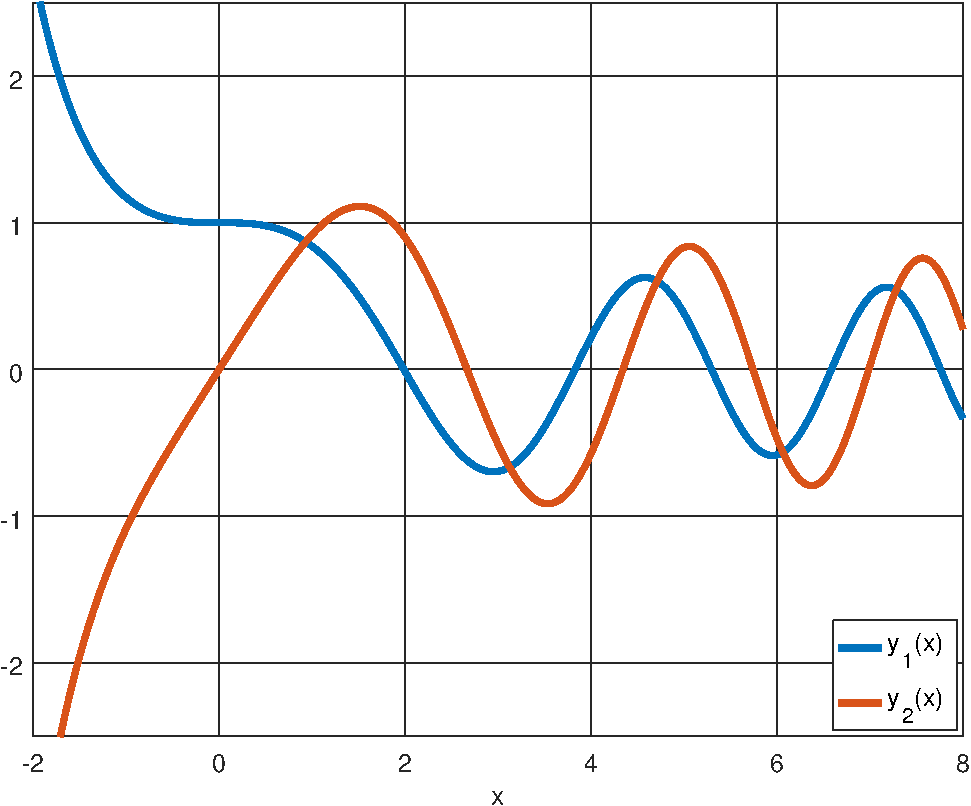
\includegraphics[width=0.5\textwidth]{figs/airyplots}
\end{frame}


\begin{frame}[fragile]
\frametitle{Airy equation 3}

\begin{itemize}
\item X
\end{itemize}

\begin{Verbatim}[fontsize=\scriptsize]
% PLOTAIRY  Plot approximations to two linearly-independent solutions to
% Airy's equation
%    y'' + x y = 0

x = -2:.01:2;
y1n12 = 1 - (1/(3*2))*x.^3 + (1/(6*5*3*2))*x.^6 - (1/(9*8*6*5*3*2))*x.^9 ...
        + (1/(12*11*9*8*6*5*3*2))*x.^12;
y2n13 = x - (1/(4*3))*x.^4 + (1/(7*6*4*3))*x.^7 - (1/(10*9*7*6*4*3))*x.^10 ...
        + (1/(13*12*10*9*7*6*4*3))*x.^13;

plot(x,y1n12,x,y2n13)
grid on,  xlabel x,  legend('y_1(x)','y_2(x)')
\end{Verbatim}
\end{frame}


\begin{frame}{you will see problem like this on quiz!}

\noindent \emph{exercise.}  for $y''-3y'-4y=0$,

\begin{itemize}
\item[(a)] solve by any means you want
\item[(b)] solve by series
\end{itemize}

\vspace{50mm}
\end{frame}


\begin{frame}{ordinary versus singular}

\begin{itemize}
\item X
\end{itemize}
\end{frame}


\begin{frame}{like exercise \#2 in \S 6.2}

\noindent \emph{exercise.}  without actually solving the DE, find the minimum radius of convergence of the power series solutions \emph{(a)} about the ordinary point $x=0$, and \emph{(b)} about the ordinary point $x=2$:
    $$(x^2+1) y'' - 6 y = 0$$

\vspace{50mm}
\end{frame}


\begin{frame}{exercise \#16 in \S 6.2}

\noindent \emph{exercise.}  find two power series solutions about $x=0$:
    $$(x^2+1) y'' - 6 y = 0$$

\vspace{50mm}
\end{frame}


\begin{frame}{exercise \#21 in \S 6.2}

\noindent \emph{exercise.}  use power series to solve the IVP:
    $$y'' - 2 x y' + 8 y = 0, \quad y(0)=3, \, y'(0)=0$$

\vspace{50mm}
\end{frame}


\begin{frame}{expectations}

\begin{itemize}
\item just watching this video is \emph{not} enough!
     \begin{itemize}
     \item see ``found online'' videos at

     \centerline{\href{https://bueler.github.io/math302/week9.html}{\tt \color{cyan} bueler.github.io/math302/week9.html}}
     \item \emph{read} section 6.2 in the textbook
     \item \emph{do} the WebAssign exercises for section 6.2
     \end{itemize}
\end{itemize}
\end{frame}

\end{document}

